\documentclass[english,xcolor=svgnames]{beamer}

\input{../../../../Templates/Latex/teachingslidesbeamer.tex}


% ===========================================================
% ===========================================================
% ===========================================================
\begin{document}

\title{New Keynesian Model}
\vspace{1cm}
\author[shortname]{
\begin{tabular}{c}
	Johannes Wieland \\ 
	\footnotesize \href{mailto:jfwieland@ucsd.edu}{jfwieland@ucsd.edu}  \\ 
\end{tabular}
}

\date{Spring \the\year}

\setbeamertemplate{footline}{}
\makebeamertitle
\setbeamertemplate{footline}[frame number]{}

\addtocounter{framenumber}{-1}


%\begin{frame}
%\frametitle{Todo}
%\begin{itemize}
%	\item Skip all the log-linearization
%	\item Write model in terms of levels, not gaps
%	\item Set $\gamma=1$ and $\alpha=0$ (earlier lectures).
%\end{itemize}
%\end{frame}

%%%%%%%%%%%%%%%%%%%%%%%%%%%%%%%%%%%%%%%%%%%%%%%%%%
\AtBeginSection[]{
\setbeamertemplate{footline}{}
  \frame<beamer>{ 

    \frametitle{Outline}   

    \tableofcontents[currentsection] 
  }
\setbeamertemplate{footline}[frame number]{}
\addtocounter{framenumber}{-1}
}

\AtBeginSubsection[]{
\setbeamertemplate{footline}{}
  \frame<beamer>{ 

    \frametitle{Outline}   

    \tableofcontents[currentsection,currentsubsection] 
  }
  \setbeamertemplate{footline}[frame number]{}
  \addtocounter{framenumber}{-1}
}


%\begin{frame}
%\frametitle{New Keynesian Model: Outline}
%\begin{enumerate}[1.]
%	\item The Baseline New Keynesian Model
%	\begin{enumerate}[{1.}1]
%		\item Setup
%		\item Nonlinear Equations: Intuition
%		\item Log-Linearized Version
%		\item The Three Equation Model
%		\item Calibrated Model: Impulse Responses and Intuition
%	\end{enumerate}
%	\item Early Critiques of the New Keynesian Model
%	\begin{enumerate}[2.1.]
%		\item Credible Disinflation
%		\item Sticky Inflation and Responses
%	\end{enumerate}
%	\item Medium-Scale NK Models
%	\item Recent Critiques and Tests of the New Keynesian Model
%	\begin{enumerate}[4.1.]
%		\item The Minnesota Critique
%		\item The Cochrane Critique: Taylor Rule and Indeterminacy
%		\item The New Keynesian Phillips Curve in the Data
%	\end{enumerate}
%\end{enumerate}
%\end{frame}

%%%%%%%%%%%%%%%%%%%%%%%%%%%%%%%%%%%%%%%%%%%%%%%%%%
\section{Introduction}
%%%%%%%%%%%%%%%%%%%%%%%%%%%%%%%%%%%%%%%%%%%%%%%%%%


%\begin{frame}
%\frametitle{New Keynesian Model: Roadmap}
%\begin{itemize}
%	\item The textbook New Keynesian model includes:
%	\begin{enumerate}[1.]
%		\item Money (in the utility function)
%		\item Monopolistic Competition
%		\item Nominal Rigidities
%	\end{enumerate}
%	\item We have been introducing these ingredients one by one.
%	\item Last class, discussed simple, one-period nominal rigidity which
%gives some intuition.
%	\begin{itemize}
%		\item Price is markup over expected marginal cost.
%		\item When marginal cost rises, markups fall. This happens with a
%monetary expansion.
%		\item Technology shocks reduce hours worked because aggregate
%demand is predetermined.
%	\end{itemize}
%	\item Today, add more persistent price stickiness.
%\end{itemize}
%\end{frame}



\begin{frame}
\frametitle{New Keynesian Model: Roadmap}
\begin{itemize}
	\item Three ``blocks'' to the model:
\end{itemize}
\begin{enumerate}[1.]
	\item Household: Same as in money model.
	\begin{itemize}
		\item Optimality conditions generate ``Dynamic IS'' curve that gives relationship between output and real interest rate.
	\end{itemize}
	\item Firms: Same as imperfect competition model, with addition of persistent nominal rigidity for intermediate producers.
	\begin{itemize}
		\item Generates a ``New Keynesian Phillips Curve,'' a forward-looking, expectations-augmented Phillips curve.
	\end{itemize}
	\item Monetary authority's nominal interest rate rule closes model.
\end{enumerate}
\end{frame}

%%%%%%%%%%%%%%%%%%%%%%%%%%%%%%%%%%%%%%%%%%%%%%%%%%
\section{New Keynesian Model}
%%%%%%%%%%%%%%%%%%%%%%%%%%%%%%%%%%%%%%%%%%%%%%%%%%



\begin{frame}
\frametitle{Household Problem: }
\begin{align*}
	\max_{\{C_t,N_t,B_t,M_t\}} & E_t \left\{\sum_{s=0}^{\infty}\beta^s\left(\frac{C_{t+s}^{1-\gamma}}{1-\gamma}+\zeta\frac{(M_{t+s}/P_{t+s})^{1-\nu}}{1-\nu}-\chi \frac{N_{t+s}^{1+\varphi}}{1+\varphi}\right)\right\} \\
	C_{t}&=\frac{W_t}{P_t}N_t-\frac{B_t-Q_{t-1}B_{t-1}}{P_t}-\frac{M_t-M_{t-1}}{P_t}+TR_t+PR_t
\end{align*}
\begin{itemize}
\item FOC
\begin{align*}
	\frac{W_t}{P_t}&=\frac{\chi N_t^\varphi}{C_t^{-\gamma}} \\
	\frac{M_t}{P_t}&=\zeta^{1/\nu}\left(1-\frac{1}{Q_t}\right)^{-1/\nu}C_{t}^{\gamma/\nu}\\
	1&=\beta E_t\left\{Q_t \frac{P_t}{P_{t+1}} \frac{C_{t+1}^{-\gamma}}{C_{t}^{-\gamma}}\right\}=E_{t}\{\Lambda_{t,t+1}R_{t+1}\}\\
\end{align*}
plus Fisher: $E_{t}\{R_{t+1}\}\equiv E_{t}\{Q_tP_t/P_{t+1}\}$
\end{itemize}
\end{frame}

\begin{frame}
\frametitle{Firm Problem
}
\begin{itemize}
	\item From the firm problem we derived the optimal price when able to adjust:
	\begin{align*}
		P_t^* &=  (1+\mu)E_t\left\{\sum_{s=0}^{\infty}\frac{\theta^s\Lambda_{t,t+s}Y_{t+s}P_{t+s}^{\epsilon-1}}{\sum_{k=0}^{\infty}\theta^k\Lambda_{t,t+k}Y_{t+k}P_{t+k}^{\epsilon-1}}\frac{W_{t+s}}{A_{t+s}}\right\} 
	\end{align*}
	\item And the price level is a geometric average of past and new prices:
	\begin{align*}
		P_t&=\left[\theta P_{t-1}^{1-\epsilon} + (1-\theta) P_{t}^{*1-\epsilon}\right]^{\frac{1}{1-\epsilon}} \\
	\end{align*}
\end{itemize}
\end{frame}


\begin{frame}
\frametitle{Interest Rate Rule
}
\begin{itemize}
	\item The central bank sets the nominal rate following an interest rate rule
	\begin{align*}
		Q_t = \beta^{-1}\left(\frac{P_t}{P_{t-1}}\right)^{\phi_{\pi}}e^{v_t},\qquad \phi_\pi, \ge 0 \\
	\end{align*}
	where $v_t$ is a ``monetary policy shock''.
%	$v_t=\rho_v v_{t-1}+\epsilon_t^v$ follows an AR(1) process.
	\begin{itemize}
		\item Central bank raises nominal rate in response to inflation, $\Pi_t=(P_t/P_{t-1})$.
		\item Viewed as a realistic description of central bank behavior in practice (Taylor, 1993). Also known as ``Taylor rule.''
		\item More realistic versions also feature interest rate smoothing and response to output gap / growth.
		\item Could alternatively solve for optimal monetary policy rule---we will do that soon.
		\item Ignores zero lower bound constraint.
	\end{itemize}
%	\item Because the central bank directly sets $Q_t$, $M_t$ is determined
\end{itemize}
\end{frame}

\begin{frame}
\frametitle{New Keynesian Model Equilibrium
}
A symmetric equilibrium is an allocation $\{C_{t+s}, N_{t+s},Y_{t+s}\}_{s=0}^{\infty}$ and
set of prices $\{P_{t+s}^*, P_{t+s},W_{t+s},Q_{t+s}\}_{s=0}^{\infty}$ along with exogenous processes $\{A_{t+s},v_{t+s}\}_{s=0}^{\infty}$ such that:
\begin{enumerate}[1.]
	\item Households optimize: Euler, labor-leisure, (money demand in background as central bank chooses $Q_{t+s}$, putting $B_{t+s}$ in background as well).
	\item Firms optimize:
	\begin{enumerate}[2.1]
		\item Price index follows dynamic Calvo formulation.
		\item Intermediate reset prices are chosen optimally.
	\end{enumerate}
	\item Central bank follows interest rate rule with shock $v_t$.
	\item Labor and goods (and bond) markets clear.
\end{enumerate}
\end{frame}

%\section{Nonlinear Equations: Intuition}

\begin{frame}
\frametitle{Equilibrium: Nonlinear Equations
}
\begin{align*}
	\frac{W_t}{P_t}&=\frac{\chi N_t^\varphi}{C_t^{-\gamma}} \\
	1&=\beta E_t\left\{Q_t \frac{P_t}{P_{t+1}} \frac{C_{t+1}^{-\gamma}}{C_{t}^{-\gamma}}\right\}=E_{t}\{\Lambda_{t,t+1}R_{t+1}\} \\
	P_t&=\left[\theta P_{t-1}^{1-\epsilon} + (1-\theta) P_{t}^{*1-\epsilon}\right]^{\frac{1}{1-\epsilon}} \\
	P_t^* &=  (1+\mu)E_t\left\{\sum_{s=0}^{\infty}\frac{\theta^s\Lambda_{t,t+s}Y_{t+s}P_{t+s}^{\epsilon-1}}{\sum_{k=0}^{\infty}\theta^k\Lambda_{t,t+k}Y_{t+k}P_{t+k}^{\epsilon-1}}\frac{W_{t+s}}{A_{t+s}}\right\} \\
	Y_t&=C_t \\
Y_t&=A_tN_t\left[\int_0^1\left(\frac{N_t(i)}{N_t}\right)^{\frac{\epsilon-1}{\epsilon}}di\right]^{\frac{\epsilon}{\epsilon-1}} \\
	Q_t &= \beta^{-1}\left(\frac{P_t}{P_{t-1}}\right)^{\phi_{\pi}}e^{v_t}
\end{align*}
\end{frame}

%\begin{frame}
%\frametitle{Nonlinear Equations: Intuition
%}
%\begin{itemize}
%	\item Before log-linearizing, intuition from nonlinear equations.
%	\item Combining $MC_t$ with $Y_t = C_t$ and labor-leisure gives:
%	\begin{align*}
%		P_t MC_t = \frac{W_{t}}{A_t} = \frac{\chi N_t^{\varphi}/C_{t}^{-\gamma}P_t}{Y_t/N_t}=\chi\frac{N_t^{1+\varphi }P_t}{Y_t^{1-\gamma}}
%	\end{align*}
%	\begin{itemize}
%		\item Approximation from assuming $Y_t = A_t N_t$ and ignoring the
%effect of $N_t(i)$ dispersion on $Y_t$ (which is second order).
%	\end{itemize}
%	\item Plug into $P^*$ and use $\Lambda_{t,t+s}=\beta\frac{C_{t+s}^{-\gamma}}{C_{t}^{-\gamma}}$ to obtain:
%	\begin{align*}
%		P_t^* &=  \chi(1+\mu)E_t\left\{\sum_{s=0}^{\infty}\frac{(\theta\beta)^s \frac{C_{t+s}^{-\gamma}}{C_{t}^{-\gamma}}Y_{t+s}P_{t+s}^{\epsilon-1}}{\sum_{k=0}^{\infty}(\theta\beta)^k \frac{C_{t+k}^{-\gamma}}{C_{t}^{-\gamma}}Y_{t+k}P_{t+k}^{\epsilon-1}}\frac{N_{t+s}^{1+\varphi }P_{t+s}}{Y_{t+s}^{1-\gamma}}\right\} \\
%		&=\chi(1+\mu)E_t\left\{\sum_{s=0}^{\infty}\frac{(\theta\beta)^s P_{t+s}^{\epsilon-1} N_{t+s}^{1+\varphi }P_{t+s}}{\sum_{k=0}^{\infty}(\theta\beta)^k Y_{t+k}^{1-\gamma} P_{t+k}^{\epsilon-1}}\right\} 
%	\end{align*}
%\end{itemize}
%\end{frame}
%
%
%\begin{frame}
%\frametitle{Nonlinear Equations: Forward Looking Price Setting
%}
%\begin{align*}
%	P_t^*&=\chi(1+\mu)E_t\left\{\sum_{s=0}^{\infty}\frac{(\theta\beta)^s P_{t+s}^{\epsilon-1} N_{t+s}^{1+\varphi }P_{t+s}}{\sum_{k=0}^{\infty}(\theta\beta)^k Y_{t+k}^{1-\gamma} P_{t+k}^{\epsilon-1}}\right\} 
%\end{align*}
%\begin{itemize}
%	\item $P_t^*$, and hence inflation, \emph{is increasing in future $P_{t+s}$} and thus
%future inflation.
%	\begin{itemize}
%		\item The $P_{t+s}$ term comes from nominal marginal costs.
%		\item Labor-leisure condition implies that real wage = MRS.
%		\item If inflation is expected to be higher, must pay higher nominal
%wage to hire labor, and nominal marginal costs will rise.
%		\item Set higher price today to cover the average discounted nominal
%marginal cost until can change price again.
%	\end{itemize}
%	\item \emph{Price setting is forward looking and incorporates expected future inflation.}
%\end{itemize}
%\end{frame}
%
%
%\begin{frame}
%\frametitle{Nonlinear Equations: Flexible Price Equilibrium
%}
%\begin{itemize}
%	\item Shut down expected future inflation: $P_{t+s} = P_{t+s-1} \;\forall s>0$.
%	\item Consider price setting in a flexible price equilibrium:
%	\begin{align*}
%		P_t^* &=  \chi(1+\mu)\frac{N_{t}^{1+\varphi }P_{t}}{Y_{t}^{1-\gamma}} \\
%		Y_{t}^{1-\gamma}&=\chi(1+\mu)N_t^{1+\varphi}
%	\end{align*}
%	\item If in flex price equilibrium, the economy-wide marginal cost is constant.
%	\begin{align*}
%		1=\frac{P_t^*}{P_t}=(1+\mu)MC_t
%	\end{align*}
%	\item Suppose one firm is subject to Calvo pricing:
%	\begin{align*}
%		P_t^*\approx P_t \times E_t\left\{\sum_{s=0}^{\infty}\frac{(\theta\beta)^s Y_{t+s}^{1-\gamma } P_{t+s}^{\epsilon-1} }{\sum_{k=0}^{\infty}(\theta\beta)^k Y_{t+k}^{1-\gamma} P_{t+k}^{\epsilon-1}}\right\} = P_t
%	\end{align*}
%\end{itemize}
%\end{frame}
%
%
%\begin{frame}
%\frametitle{Nonlinear Equations: Flexible Price Equilibrium
%}
%\begin{align*}
%		P_t^*\approx P_t \times E_t\left\{\sum_{s=0}^{\infty}\frac{(\theta\beta)^s Y_{t+s}^{1-\gamma } P_{t+s}^{\epsilon-1} }{\sum_{k=0}^{\infty}(\theta\beta)^k Y_{t+k}^{1-\gamma} P_{t+k}^{\epsilon-1}}\right\} = P_t
%	\end{align*}
%\begin{itemize}
%	\item If at flexible price level of output and do not expect future inflation, no inflation today because resetters choose to mimic flexible price.
%	\begin{itemize}
%		\item In flexible price equilibrium, marginal costs are constant and the average mark-up is at the desired level.
%		\item  And there is no expected inflation.
%		\item So resetters set their markup equal to average markup and
%there is no inflation.
%	\end{itemize}
%\end{itemize}
%\end{frame}
%
%
%\begin{frame}
%\frametitle{Nonlinear Equations: Phillips Curve
%}
%\begin{itemize}
%	\item Putting everything together, the NK model features an \emph{expectations-augmented Phillips curve}.
%	\begin{itemize}
%		\item Because price setting is forward looking, Phillips curve is going to be \emph{expectation-augmented}.
%		\item Output-inflation relationship relates inflation to deviations from flex price output (called the \emph{natural level of output}).
%		\begin{itemize}
%			\item At natural level of output with no expected inflation, resetters choose price equal to flexible price, resulting in no inflation.
%			\item If output deviates, that is if the output gap $\tilde{Y}_t = (Y_t-Y_t^{flex})/Y_t^{flex}$ is nonzero, the extra output will bid up nominal wages and move marginal costs, causing inflation in response to deviations of output from its flexible level.
%		\end{itemize}
%	\end{itemize}
%	\item NK model a response to Lucas Critique.
%	\begin{itemize}
%		\item Unlike ``old'' Keynesian models, only unexpected inflation moves output.
%		\item Central bank cannot regularly exploit output-inflation trade-off.
%	\end{itemize}
%\end{itemize}
%\end{frame}
%
%
%\begin{frame}
%\frametitle{Nonlinear Equations: Labor Wedge
%}
%\begin{itemize}
%	\item Note that for firm with markup $\mu_t(i)$,
%	\begin{align*}
%		1+\mu_t(i)=\frac{P_t(i)/P_t}{MC_t}
%	\end{align*}
%	\item But on average, $P_t (i)/P_t=1$ so
%	\begin{align*}
%		1+\mu_t=\frac{1}{MC_t}=\frac{Y_t/N_t}{W_t/P_t}=\frac{MPL_t}{MRS_t}
%	\end{align*}
%	\item So the labor wedge is the average markup, which is countercyclical.
%\end{itemize}
%\end{frame}



%%%%%%%%%%%%%%%%%%%%%%%%%%%%%%%%%%%%%%%%%%%%%%%%%%
\section{Log Linearization}
%%%%%%%%%%%%%%%%%%%%%%%%%%%%%%%%%%%%%%%%%%%%%%%%%%


\begin{frame}
\frametitle{Log Linearization
}
%\begin{itemize}
%	\item Philips curve should be function of output gap, so want to write whole model as function of output gap.
%	\item Strategy:
	\begin{itemize}
		\item  Log-Linearize Model Around \emph{Zero-Inflation Steady State}.
		\begin{enumerate}[1.]
			\item AD Block: Euler Equation $\Rightarrow$ \emph{Dynamic IS Curve}
			\item AS Block: Pricing and MC Equations $\Rightarrow$ NK Phillips Curve
			\item Central Bank Monetary Rule
		\end{enumerate}
%		\item Log-Linearize Flex Price Equilibrium.
%		\item Difference To Get Equilibrium In Terms of Output Gap.
	\item Why log-linearize?
	\begin{itemize}
		\item Much(!!!!) easier to analyze and understand linear system than non-linear model.
	\end{itemize}
	\item I will skip most of the log-linearization.
	\begin{itemize}
		\item Life is short---see Gali for details.
		\item Focus on economics of NK model.
	\end{itemize}
	\end{itemize}
%\end{itemize}
\end{frame}


%\begin{frame}
%\frametitle{Log Linearization: The Aggregate Supply Block}
%\begin{align*}
%	\frac{W_t}{P_t}&=\frac{\chi N_t^\varphi}{C_t^{-\gamma}} \\
%%	1&=\beta E_t\left\{Q_t \frac{P_t}{P_{t+1}} \frac{C_{t+1}^{-\gamma}}{C_{t}^{-\gamma}}\right\}=E_{t}\{\Lambda_{t,t+1}R_{t+1}\} \\
%	P_t&=\left[\theta P_{t-1}^{1-\epsilon} + (1-\theta) P_{t}^{*1-\epsilon}\right]^{\frac{1}{1-\epsilon}} \\
%	P_t^* &=  (1+\mu)E_t\left\{\sum_{s=0}^{\infty}\frac{\theta^s\Lambda_{t,t+s}Y_{t+s}P_{t+s}^{\epsilon-1}}{\sum_{k=0}^{\infty}\theta^k\Lambda_{t,t+k}Y_{t+k}P_{t+k}^{\epsilon-1}}\frac{W_{t+s}}{A_{t+s}}\right\} \\
%%	Y_t&=C_t \\
%Y_t&=A_tN_t\left[\int_0^1\left(\frac{N_t(i)}{N_t}\right)^{\frac{\epsilon-1}{\epsilon}}di\right]^{\frac{\epsilon}{\epsilon-1}} 
%%\\
%%	Q_t &= \beta^{-1}\left(\frac{P_t}{P_{t-1}}\right)^{\phi_{\pi}}\left(\frac{Y_t}{\bar{Y}}\right)^{\phi_{y}}e^{v_t}
%\end{align*}
%\begin{itemize}
%	\item Labor-leisure:
%	\begin{align*}
%		\hat{w}_t-\hat{p}_t=\varphi\hat{n}_t+\gamma\hat{c}_t
%	\end{align*}
%	\item Production function:
%	\begin{align*}
%		\hat{y}_t=\hat{a}_t+\hat{n}_t
%	\end{align*}
%\end{itemize}
%\end{frame}

\begin{frame}
\frametitle{Log Linearization}
\begin{itemize}
	\item Log-linear approximation of $Y_t = f (X_t )$ around a point $X$ .
	\begin{itemize}
		\item First-order Taylor approx to $\log (f(X))$
	\end{itemize}
	\item Define $x_t=\log(X_t)$ and $\hat{x}_t = x_t-x$.
	\begin{align*}
		y_t &= \log (f(\exp(x_t))) \\
		 &\approx \log (f(\exp(x))) +  \frac{f'(\exp(x))\exp(x)}{f(\exp(x))}(x_t-x) \\
		 \hat{y}_t &\approx \frac{f'(X)X}{f(X)}\hat{x}_t
	\end{align*}
	\item Can also derive using $\hat{x}_t\approx\frac{X_t-X}{X}\equiv\frac{dX_t}{X}$
	\begin{align*}
		Y + dY_t &= f(X)+f'(X)dX_t \\
		\frac{dY_t}{Y}Y &= f'(X)X\frac{dX_t}{X} \\
		\hat{y}_t &\approx \frac{f'(X)X}{f(X)}\hat{x}_t
	\end{align*}
\end{itemize}
\end{frame}

\begin{frame}
\frametitle{Log Linearization: Inflation
}
\begin{itemize}
	\item Price Index:
	\begin{align*}
		P_t&=\left[\theta P_{t-1}^{1-\epsilon} + (1-\theta) P_{t}^{*1-\epsilon}\right]^{\frac{1}{1-\epsilon}} 
	\end{align*}
	\item The price index can be log-linearized to get
	\begin{align*}
		\hat{p}_t=\theta \hat{p}_{t-1}+(1-\theta)\hat{p}_t^*
	\end{align*}
	\begin{itemize}
		\item Equivalently written in terms of inflation:
		\begin{align*}
		\hat{\pi}_t=(1-\theta)(\hat{p}_t^*-\hat{p}_{t-1})
	\end{align*}
	\item Inflation is positive when new prices are higher than old prices.
	\end{itemize}
\end{itemize}
\end{frame}


\begin{frame}
\frametitle{Log Linearization: Reset Prices
}
\begin{itemize}
	\item The reset price can be log-linearized as:
	\begin{align*}
		\hat{p}_t^*=(1-\beta\theta)E_t\left\{\sum_{s=0}^{\infty}(\beta\theta)^s\left(\hat{p}_{t+s}+\hat{mc}_{t+s}\right)\right\} 
	\end{align*}
	\item We can write this recursively as:
	\begin{align*}
		\hat{p}_t^*=(1-\beta\theta)(\hat{p}_{t}+\hat{mc}_{t})+\beta\theta E_t\{\hat{p}_{t+1}^*\}
	\end{align*}
\end{itemize}
\end{frame}


\begin{frame}
\frametitle{Log Linearization: Phillips Curve
}
\begin{itemize}
	\item Subtract $\hat{p}_{t-1}$:
	\begin{align*}
		(\hat{p}_t^*-\hat{p}_{t-1})=(1-\beta\theta)\hat{mc}_{t}+\hat{\pi}_t+\beta\theta E_t\{\hat{p}_{t+1}^*-\hat{p}_{t}\}
	\end{align*}
	\item Plug into $\hat{\pi}_t=(1-\theta)(\hat{p}_t^*-\hat{p}_{t-1})$ to get an expectations-augmented Phillips curve:
	\begin{align*}
		\hat{\pi}_t=\lambda\hat{mc}_{t}+\beta E_t\{\hat{\pi}_{t+1}\},\;\text{ where }\;\lambda=\frac{(1-\theta)(1-\beta\theta)}{\theta}
	\end{align*}
	\item Inflation is equal to expected future inflation plus the deviation of marginal cost from its steady state level.
	\begin{itemize}
		\item Expected inflation: Forward looking price setters choose higher prices now if inflation is expected to be high, as nominal marginal costs will rise.
	\end{itemize}
\end{itemize}
\end{frame}


\begin{frame}
\frametitle{Log Linearization: Phillips Curve
}
\begin{itemize}
	\item Inflation is equal to expected future inflation plus the deviation of marginal cost from its steady state level.
	\begin{itemize}
		\item Two ways to think about marginal cost deviation:
	\end{itemize}
	\begin{enumerate}[1.]
		\item Set higher prices to cover higher marginal cost.
		\item When marginal costs are above desired level, markups are
below desired level. Inflation as firms hike markup back to desired level. (In fact, $\hat{mc}_t = -\hat{\mu}_t$).
	\end{enumerate}
	\item Iterating forward,
	\begin{align*}
		\hat{\pi}_t=\lambda E_t\left\{\sum_{s=0}^{\infty}\beta^s\hat{mc}_{t+s}\right\}
	\end{align*}
	\begin{itemize}
		\item Inflation is the PDV of future marginal cost / markup deviations from steady state.
	\end{itemize}
\end{itemize}
\end{frame}


\begin{frame}
\frametitle{Log Linearization: Real Marginal Costs
}
\begin{align*}
	\hat{mc}_t=\hat{w}_t-\hat{p}_t-\hat{a}_t
\end{align*}
\begin{itemize}
	\item Combine labor-leisure, production function, and $\hat{c}_t=\hat{y}_t$:
	\begin{align*}
		\hat{w}_t-\hat{p}_t=(\gamma+\varphi)\hat{y}_t-\varphi\hat{a}_t
\end{align*}
	\item Consequently,
	\begin{align*}
	\hat{mc}_t=(\gamma+\varphi)\hat{y}_t-(1+\varphi)\hat{a}_t
\end{align*}
\item Compare to flexible price case:
\begin{align*}
	1 = \frac{P_t(i)}{P_t} = \mu\frac{W_t}{P_t}\frac{1}{A_t} 
\end{align*}
so
\begin{align*}
	\hat{mc}_t^{flex} = 0,\qquad (\gamma+\varphi)\hat{y}_t^{flex}&=(1+\varphi)\hat{a}_t \\
\end{align*}
where $\hat{y}_t^{flex}$ is called the \emph{natural level of output}.
\end{itemize}
\end{frame}


%\begin{frame}
%\frametitle{Nonlinear Equations: Phillips Curve
%}
%\begin{itemize}
%	\item Putting everything together, the NK model features an \emph{expectations-augmented Phillips curve}.
%	\begin{itemize}
%		\item Because price setting is forward looking, Phillips curve is going to be \emph{expectation-augmented}.
%		\item Output-inflation relationship relates inflation to deviations from flex price output (called the \emph{natural level of output}).
%		\begin{itemize}
%			\item At natural level of output with no expected inflation, resetters choose price equal to flexible price, resulting in no inflation.
%			\item If output deviates, that is if the output gap $\tilde{Y}_t = (Y_t-Y_t^{flex})/Y_t^{flex}$ is nonzero, the extra output will bid up nominal wages and move marginal costs, causing inflation in response to deviations of output from its flexible level.
%		\end{itemize}
%	\end{itemize}
%	\item NK model a response to Lucas Critique.
%	\begin{itemize}
%		\item Unlike ``old'' Keynesian models, only unexpected inflation moves output.
%		\item Central bank cannot regularly exploit output-inflation trade-off.
%	\end{itemize}
%\end{itemize}
%\end{frame}


%\begin{frame}
%\frametitle{Log Linearization: Flexible Price Equilibrium
%}
%\begin{align*}
%	\frac{W_t^{flex}}{P_t^{flex}}&=\frac{\chi (N_t^{flex})^\varphi}{(C_t^{flex})^{-\gamma}} \\
%%	1&=\beta E_t\left\{Q_t \frac{P_t}{P_{t+1}} \frac{C_{t+1}^{-\gamma}}{C_{t}^{-\gamma}}\right\}=E_{t}\{\Lambda_{t,t+1}R_{t+1}\} \\
%%	P_t&=\left[\theta P_{t-1}^{1-\epsilon} + (1-\theta) P_{t}^{*1-\epsilon}\right]^{\frac{1}{1-\epsilon}} \\
%	\frac{W_t^{flex}}{P_t^{flex}} &=  \frac{A_t}{1+\mu} \\
%	Y_t^{flex}&=C_t^{flex} \\
%Y_t^{flex}&=A_t^{flex}N_t^{flex}
%%\\
%%	Q_t &= \beta^{-1}\left(\frac{P_t}{P_{t-1}}\right)^{\phi_{\pi}}\left(\frac{Y_t}{\bar{Y}}\right)^{\phi_{y}}e^{v_t}
%\end{align*}
%\begin{itemize}
%	\item Combine to get:
%	\begin{align*}
%		A_t^{1+\varphi}&=\chi(1+\mu)(Y_t^{flex})^{\gamma+\varphi} \\
%	(\gamma+\varphi)\hat{y}_t^{flex}&=(1+\varphi)\hat{a}_t
%\end{align*}
%\end{itemize}
%\end{frame}
%
\begin{frame}
\frametitle{Real Marginal Costs in Terms of Output Gap
}
\begin{itemize}
	\item Combine:
	\begin{align*}
		\hat{mc}_t&=(\gamma+\varphi)\hat{y}_t-(1+\varphi)\hat{a}_t \\
		(\gamma+\varphi)\hat{y}_t^{flex}&=(1+\varphi)\hat{a}_t \\
\end{align*}
	to write real marginal costs in terms of output gap $\tilde{y}_t$:
	\begin{align*}
		\hat{mc}_t&=(\gamma+\varphi)(\hat{y}_t-\hat{y}_t^{flex})
	\end{align*}
	\item Real marginal costs go up (and markups go down) when the output gap is high.
	\begin{itemize}
		\item To produce more than under flex prices, markup must be lower.
		\item Marginal costs high because need to hire more workers,
bidding up real wage.
		\item Stronger when IES and labor supply elasticity are low.
		\item In Gali textbook also stronger with DRS.
	\end{itemize}
\end{itemize}
\end{frame}

%
%\begin{frame}
%\frametitle{The New Keynesian Phillips Curve
%}
%\begin{itemize}
%	\item Plug back into the Phillips curve $\hat{\pi}_t=\lambda\hat{mc}_{t}+\beta E_t\{\hat{\pi}_{t+1}\}$
%	\begin{align*}
%		\hat{\pi}_t=\kappa\tilde{y}_t+\beta E_t\{\hat{\pi}_{t+1}\},\;\text{ where }\;\kappa=\lambda(\gamma+\varphi)
%\end{align*}
%	\begin{itemize}
%		\item This is the \emph{New Keynesian Philips Curve}: an expectations augmented Phillips curve written in terms of the output gap.
%	\end{itemize}
%	\item Solving forward,
%	\begin{align*}
%		\hat{\pi}_t=\kappa E_t\left\{\sum_{s=0}^{\infty}\beta^s\tilde{y}_{t+s}\right\}
%	\end{align*}
%	\begin{itemize}
%		\item Inflation is an increasing function of future output gaps.
%		\item Output gap high $\Rightarrow$ marginal cost high and markups low $\Rightarrow$ raise markups.
%	\end{itemize}
%\end{itemize}
%\end{frame}


\begin{frame}
\frametitle{The New Keynesian Phillips Curve
}
\begin{itemize}
	\item Plug back into the Phillips curve $\hat{\pi}_t=\lambda\hat{mc}_{t}+\beta E_t\{\hat{\pi}_{t+1}\}$
	\begin{align*}
		\hat{\pi}_t=\kappa(\hat{y}_t-\hat{y}_t^{flex})+\beta E_t\{\hat{\pi}_{t+1}\},\;\text{ where }\;\kappa=\lambda(\gamma+\varphi)
\end{align*}
	\begin{itemize}
		\item This is the \emph{New Keynesian Philips Curve}: an expectations augmented Phillips curve written in terms of the output gap.
	\end{itemize}
	\item Solving forward,
	\begin{align*}
		\hat{\pi}_t=\kappa E_t\left\{\sum_{s=0}^{\infty}\beta^s(\hat{y}_{t+s}-\hat{y}_{t+s}^{flex})\right\}
	\end{align*}
	\begin{itemize}
		\item Inflation is an increasing function of future output gaps.
		\item Output gap high $\Rightarrow$ marginal cost high and markups low $\Rightarrow$ raise markups.
	\end{itemize}
\end{itemize}
\end{frame}


%%%%%%%%%%%%%%%%%%%%%%%%%%%%%%%%%%%%%%%%%%%%%%%%%%
%\section{AD Block}
%%%%%%%%%%%%%%%%%%%%%%%%%%%%%%%%%%%%%%%%%%%%%%%%%%

\begin{frame}
\frametitle{Log Linearization: The Aggregate Demand Block
}
\begin{align*}
%	\frac{W_t}{P_t}&=\frac{\chi N_t^\varphi}{C_t^{-\gamma}} \\
	1&=\beta E_t\left\{Q_t \frac{P_t}{P_{t+1}} \frac{C_{t+1}^{-\gamma}}{C_{t}^{-\gamma}}\right\}=E_{t}\{\Lambda_{t,t+1}R_{t+1}\} \\
%	P_t&=\left[\theta P_{t-1}^{1-\epsilon} + (1-\theta) P_{t}^{*1-\epsilon}\right]^{\frac{1}{1-\epsilon}} \\
%	P_t^* &=  (1+\mu)E_t\left\{\sum_{s=0}^{\infty}\frac{\theta^s\Lambda_{t,t+s}Y_{t+s}P_{t+s}^{\epsilon-1}}{\sum_{k=0}^{\infty}\theta^k\Lambda_{t,t+k}Y_{t+k}P_{t+k}^{\epsilon-1}}\frac{W_{t+s}}{A_{t+s}}\right\} \\
	Y_t&=C_t %\\
%Y_t&=A_tN_t\left[\int_0^1\left(\frac{N_t(i)}{N_t}\right)^{\frac{\epsilon-1}{\epsilon}}di\right]^{\frac{\epsilon}{\epsilon-1}} 
%\\
%	Q_t &= \beta^{-1}\left(\frac{P_t}{P_{t-1}}\right)^{\phi_{\pi}}\left(\frac{Y_t}{\bar{Y}}\right)^{\phi_{y}}e^{v_t}
\end{align*}
\begin{itemize}
	\item Log-linearize Euler around zero-inflation:
	\begin{align*}
		\hat{c}_t=-\frac{1}{\gamma}\left(\hat{i}_t-E_t\{\hat{\pi}_{t+1}\}\right)+E_t\{\hat{c}_{t+1}\}
	\end{align*}
	\begin{itemize}
		\item Steady state nominal interest rate is $i_t = \rho = -\log \beta$.
	\end{itemize}
	\item Combine with market clearing and use $\sigma=1/\gamma$:
	\begin{align*}
		\hat{y}_t=-\sigma\left(\hat{i}_t-E_t\{\hat{\pi}_{t+1}\}\right)+E_t\{\hat{y}_{t+1}\}
	\end{align*}
	\item This is the \emph{dynamic IS curve}. It relates output to future expectations of output and the real interest rate.
\end{itemize}
\end{frame}


%\begin{frame}
%\frametitle{The Natural Rate of Interest
%}
%\begin{itemize}
%	\item Define the natural rate of interest $\hat{r}_{t+1}^n$ as the real interest rate that would prevail when output is equal to its flexible level:
%	\begin{align*}
%		\hat{y}_t^{flex}=-\sigma \hat{r}_{t+1}^n+E_t\{\hat{y}_{t+1}^{flex}\}
%	\end{align*}
%	\item Recall $\hat{y}_t^{flex}=\left(\frac{1+\varphi}{\gamma+\varphi}\right)\hat{a}_t$ so:
%	\begin{align*}
%		\hat{r}_{t+1}^n&=\gamma \frac{1+\varphi}{\gamma+\varphi}E_t\{\hat{a}_{t+1}-\hat{a}_t\} \\
%		&=\gamma \frac{1+\varphi}{\gamma+\varphi}E_t\{\Delta \hat{a}_{t+1}\} 
%	\end{align*}
%	\begin{itemize}
%		\item If $a_t$ follows an AR(1) and grows today, it will be expected to decline between today and tomorrow due to mean reversion.
%		\item So positive tech shock causes real interest rate to fall by standard RBC logic.
%	\end{itemize}
%\end{itemize}
%\end{frame}
%
%
\begin{frame}
\frametitle{Dynamic IS
}
%\begin{align*}
%		\hat{y}_t=-\sigma\left(\hat{i}_t-E_t\{\hat{\pi}_{t+1}\}\right)+E_t\{\hat{y}_{t+1}\}
%	\end{align*}
\begin{itemize}
	\item Iterating forward, the current output gap depends negatively on the gap between the real interest rate and the natural rate of interest (assuming return to steady state):
	\begin{align*}
		\hat{y}_t=-\sigma E_t\left\{\sum_{s=0}^{\infty}\left(\hat{r}_{t+s+1}\right)\right\}
	\end{align*}
	\item If you want to figure out what happens to output in the NK model, you need to figure out what happens to the path of the real interest rate.
	\begin{itemize}
		\item Output gap determined purely by intertemporal substitution. Not old Keynesian marginal propensities to consume / invest.
		\item Intuition also works well for larger NK models.
	\end{itemize}
\end{itemize}
\end{frame}

%%%%%%%%%%%%%%%%%%%%%%%%%%%%%%%%%%%%%%%%%%%%%%%%%%
\section{Three Equation Model}
%%%%%%%%%%%%%%%%%%%%%%%%%%%%%%%%%%%%%%%%%%%%%%%%%%

\begin{frame}
\frametitle{The Three Equation Model}
\begin{itemize}
	\item In sum, the log-linearized NK model boils down to three equations:
	\begin{align*}
		\hat{y}_t &=-\sigma[\hat{i}_t-E_t\{\hat{\pi}_{t+1}\}]+E_t\{\hat{y}_{t+1}\} \\
		\hat{\pi}_t&=\kappa (\hat{y}_t-\hat{y}_t^{flex}) +\beta E_t \{\hat{\pi}_{t+1}\} \\
		\hat{i}_t&=\phi_\pi\hat{\pi}_t+v_t \\
	\end{align*}
	with three unknowns: $\hat{i}_t$, $\hat{y}_t$, and $\hat{\pi}_t$  and an exogenous driving
process for the output gap $\hat{y}_t^{flex}$ ($=\frac{1+\varphi}{\gamma+\varphi}\hat{a}_t$) and the monetary policy shock $\hat{v}_t$.
	\item Key new ingredient is NK Phillips curve:
	\begin{itemize}
		\item $\beta E_t \{\hat{\pi}_{t+1}\}$: Price setters forward looking.
		\item $\kappa\hat{y}_t$: Output  $\uparrow\;\Rightarrow$ MC $\uparrow\;\Rightarrow$ markups $\downarrow\;\Rightarrow$ raise prices
	\end{itemize}
	\item Determinacy: similar condition to lecture 2. See Gali.
	\item Note: Gali writes everything in terms of ``gaps'', $\tilde{y}_t = \hat{y}_t-\hat{y}_t^{flex}$.
\end{itemize}
\end{frame}

\begin{frame}
\frametitle{Special Case: $\kappa\rightarrow\infty$}
\begin{itemize}
%	\item To understand how the NK model works let us focus first on special cases. 
	\item Equivalent to flexible prices: $\theta=0$.
	\item The NK Phillips Curve becomes:
	\begin{align*}
		\hat{y}_t = \hat{y}_t^{flex}&=\frac{1+\varphi}{\gamma+\varphi}\hat{a}_t 
	\end{align*}
	\item Output fluctuations arise only from productivity fluctuations.
	\item Monetary variables $v_t$ have no real effect:
	\begin{itemize}
		\item Drop in $v_t$ lowers nominal rate and real interest rate.
		\item All else equal increases output and marginal cost.
		\item Prices today rise with marginal cost so that $\pi_{t+1}$ is low and the real interest rate is constant.
		\item[$\Rightarrow$] With constant real interest rate output is unchanged.
	\end{itemize}
\end{itemize}
\end{frame}

\begin{frame}
\frametitle{Special Case: $\kappa=0$}
\begin{itemize}
	\item Equivalent to perfectly rigid prices: $\theta=1$.  The NK Phillips Curve becomes $\hat{\pi}_t=0$.
	\item Now output is demand determined:
	\begin{align*}
		\hat{y}_t &=-\sigma\hat{i}_t +E_t\{\hat{y}_{t+1}\} \\
		\hat{i}_t&=v_t 
	\end{align*}
	\item If $v_t = \rho_v v_{t-1}+\epsilon_t$, then
	\begin{align*}
		\hat{y}_t = -\frac{\sigma}{1-\rho_v}v_t
	\end{align*}
	\item Monetary variables $\hat{v}_t$ have a real effect:
	\begin{itemize}
		\item Drop in $v_t$ lowers nominal rate and real interest rate.
		\item Inflation is constant so output expands with the lower real interest rate.
	\end{itemize}
	\item With rigid prices, output is independent of productivity fluctuations.
\end{itemize}
\end{frame}

\begin{frame}
\frametitle{Intermediate $\kappa$}
\begin{itemize}
	\item Assume
	\begin{align*}
		v_t = \rho_v v_{t-1}+\epsilon_t \text{ and }\hat{a}_{t}=0
	\end{align*}
	\item Guess reduced form policy functions:
	\begin{align*}
		\hat{y}_t=\psi_{yv}v_t\text{ and }\hat{\pi}_t=\psi_{\pi v}v_t
	\end{align*}
	\item This gives:
	\begin{align*}
		\psi_{\pi v}&=\kappa\psi_{yv}+\beta\rho_v\psi_{\pi v}\\
		\psi_{y v}&=-\sigma(\phi_\pi \psi_{\pi v} + 1 -\rho_v \psi_{\pi v})+\rho_v \psi_{y v}
	\end{align*}
	\item Solving by method of undetermined coeffs:
	\begin{align*}
		\psi_{y v}=-(1-\beta\rho_v)\Psi_v\text{ and }\psi_{\pi v}=-\kappa \Psi_v
	\end{align*}
	\begin{align*}
		\text{where } \Psi_v=\frac{1}{(1-\beta\rho_v)\gamma(1-\rho_v)+\kappa(\phi_\pi-\rho_v)}>0
	\end{align*}
\end{itemize}
\end{frame}

\begin{frame}
\frametitle{Intermediate $\kappa$}
\centering
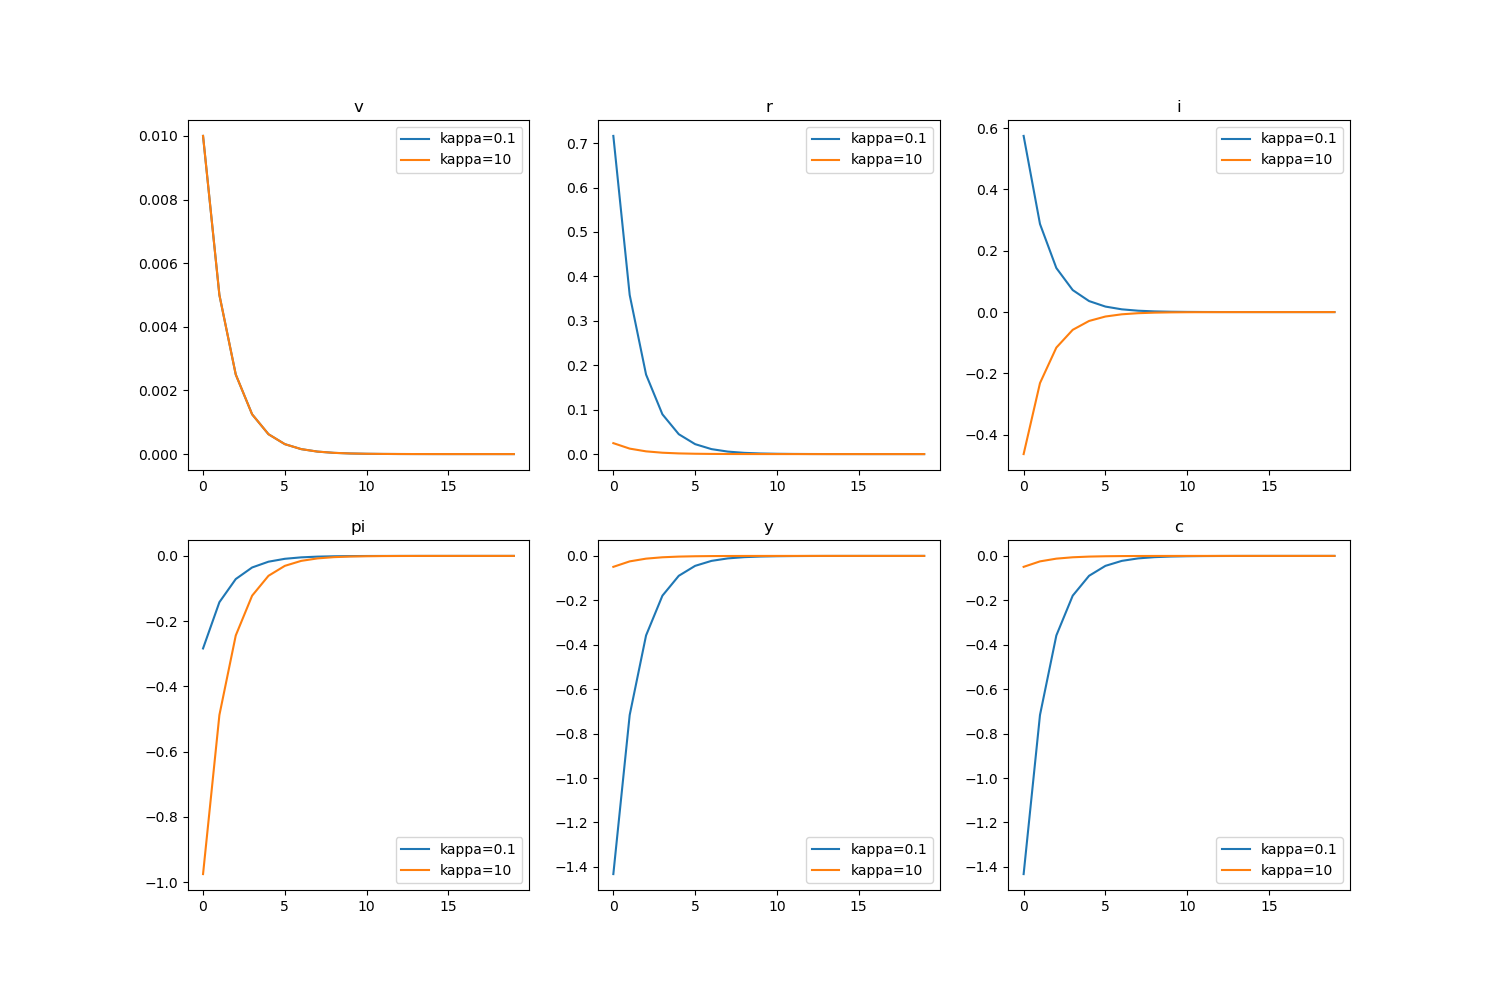
\includegraphics[scale=0.3]{nklinearirf.png}
\begin{itemize}
	\item Blue line: $\kappa = 0.1$. Orange line: $\kappa = 10$.
\end{itemize}
\end{frame}

\begin{frame}
\frametitle{Epistemiology}
\begin{itemize}
	\item NK model a response to the Lucas critique: ``fully'' optimizing agents but monetary policy has real effect.
	\item Extensive debate on how well NK model fits the data.
	\begin{itemize}
		\item Centers on much more complex ``medium-scale'' models.
		\item These are the simple NK model at its core with many additional ``bells and whistles'' (capital, habits, indexation, rigid wages, government, etc).  See references in the syllabus.
		\item Everyone agrees the simple three equation model does not match the data well.
%		\item See references in the syllabus.
	\end{itemize}
	\item Should view simple model as an organizing framework.
	\begin{itemize}
		\item Communicate results: everyone knows this model and how it works.
		\item How should policy respond to shocks? Why?
		\item Interpret policy actions through lens of NK model.
	\end{itemize}
\end{itemize}
\end{frame}

\section{Next Steps}


\begin{frame}
\frametitle{Next Steps}
\begin{itemize}
	\item Optimal policy in NK model.
	\item Interpreting Federal Reserve actions / statements through the lens of the NK model.
\end{itemize}
\end{frame}

%
%\begin{frame}
%\frametitle{Solving the Model: Monetary Policy Shocks}
%\begin{itemize}
%	\item Plug in interest rate rule and rewrite as a difference equation:
%	\begin{align*}
%		\begin{bmatrix}
%			\tilde{y}_t \\ \hat{\pi}_t
%		\end{bmatrix} = AE_t\left\{\begin{bmatrix}
%			\tilde{y}_{t+1} \\ \hat{\pi}_{t+1}
%		\end{bmatrix}\right\}+B(E_t\hat{r}_{t+1}^n-v_t)
%	\end{align*}
%	where:
%	\begin{align*}
%		A=\Omega\begin{bmatrix}
%			\gamma & 1-\beta\phi_\pi \\
%			\gamma\kappa & \kappa+\beta(\gamma+\phi_{y})
%		\end{bmatrix} \text{ and } 
%		B=\Omega\begin{bmatrix}
%			1 \\ \kappa
%		\end{bmatrix}
%	\end{align*}
%	and $\Omega=\frac{1}{\gamma+\phi_y+\kappa\phi_\pi}$.
%	\item 2 non-predetermined variables, 0 endogenous state variables.
%	\begin{itemize}
%		\item Solve forward.
%	\end{itemize}
%	\item Locally-unique bounded solution if both eigenvalues of A in unit circle:
%	\begin{align*}
%		\kappa(\phi_\pi-1)+(1-\beta)\phi_y>0 \\
%	\end{align*}
%	which holds if $\phi_{\pi}\ge 1$ and $\phi_y\ge 0$.
%	\begin{itemize}
%		\item Taylor principle still holds (and we assume it).
%	\end{itemize}
%\end{itemize}
%\end{frame}
%
%
%%\begin{frame}
%%\frametitle{Solving the Model: Monetary Policy Shocks}
%%\begin{itemize}
%%	\item Assume
%%	\begin{align*}
%%		v_t = \rho_v v_{t-1}+\epsilon_t \text{ and }\hat{r}_{t+1}^n=0
%%	\end{align*}
%%	\item Guess reduced form policy functions:
%%	\begin{align*}
%%		\tilde{y}_t=\psi_{yv}v_t\text{ and }\hat{\pi}_t=\psi_{\pi v}v_t
%%	\end{align*}
%%	\item This gives:
%%	\begin{align*}
%%		\psi_{\pi v}&=\kappa\psi_{yv}+\beta\rho_v\psi_{\pi v}\\
%%		\psi_{y v}&=-\sigma(\phi_\pi \psi_{\pi v}+\phi_y \psi_{y v} + 1 -\rho_v \psi_{\pi v})+\rho_v \psi_{y v}
%%	\end{align*}
%%	\item Solving by method of undetermined coeffs:
%%	\begin{align*}
%%		\psi_{y v}=-(1-\beta\rho_v)\Psi_v\text{ and }\psi_{\pi v}=-\kappa \Psi_v
%%	\end{align*}
%%	\begin{align*}
%%		\text{where } \Psi_v=\frac{1}{(1-\beta\rho_v)[\gamma(1-\rho_v)+\phi_y]+\kappa(\phi_\pi-\rho_v)}>0
%%	\end{align*}
%%\end{itemize}
%%\end{frame}
%
%\begin{frame}
%\frametitle{Solving the Model: Monetary Policy Shocks}
%\begin{itemize}
%	\item Contractionary monetary shock ($\uparrow v_t$) reduces $\tilde{y}_t$ and $\hat{\pi}_t$.
%	\item Consider a temporary shock ($\rho_v=0$) for intuition:
%	\begin{itemize}
%		\item By Fisher, increase in $i_t$ raises real interest rate above its natural level.
%		\item Consumption and output gap fall due to inter-temporal substitution.
%		\item Economy is aggregate demand determined so output falls.
%		\item Marginal costs fall and markups rise. Resetters cut prices to get back to desired markup. Inflation falls.
%	\end{itemize}
%\end{itemize}
%\end{frame}
%
%
%\begin{frame}
%\frametitle{Solving the Model: Technology Shocks}
%\begin{itemize}
%	\item Assume
%	\begin{align*}
%		v_t = 0\text{ and }\hat{a}_t=\rho_a \hat{a}_{t-1}+\epsilon_t^a 
%	\end{align*}
%	\item Natural rate is
%	\begin{align*}
%		\hat{r}_{t+1}^n&=\gamma \frac{1+\varphi}{\gamma+\varphi}E_t\{\Delta \hat{a}_{t+1}\} \\
%		&=-\gamma \frac{1+\varphi}{\gamma+\varphi}(1-\rho_a) \hat{a}_{t}
%	\end{align*}
%	\item $\hat{r}_{t+1}^n$ is linear function of $a$ and hence follows an AR(1) process.
%	\item And it enters with opposite sign to $v_t$, so same solution:
%	\begin{align*}
%		\tilde{y}_t=(1-\beta\rho_a)\Psi_a \hat{r}_{t+1}^n \text{ and }\hat{\pi}_t=\kappa \Psi_a \hat{r}_{t+1}^n
%	\end{align*}
%\end{itemize}
%\end{frame}
%
%\begin{frame}
%\frametitle{Solving the Model: Technology Shocks}
%\begin{itemize}
%	\item Technology shock causes output gap and inflation to fall.
%	\begin{itemize}
%		\item But flexible output rises: $\hat{y}_t^{flex}=\left(\frac{1+\varphi}{\gamma+\varphi}\right)\hat{a}_t$
%	\end{itemize}
%	\item So what happens to output and employment?
%	\begin{align*}
%		\hat{y}_t&=\hat{y}_t^{flex}+\tilde{y}_t \\
%		\hat{n}_t&=\hat{y}_t-\hat{a}_t
%	\end{align*}
%	\item If $\gamma=1$, then  $\hat{y}_t^{flex}=\hat{a}_t$ and $\hat{r}_{t+1}^n=-(1-\rho_a)\hat{a}_t$ so:
%	\begin{align*}
%		\hat{y}_t&=\rho_a(1-\beta\rho_a)\Psi_a \hat{a}_t  \\
%		\hat{n}_t&=-(1-\rho_a)(1-\beta\rho_a)\Psi_a \hat{a}_t 
%	\end{align*}
%	\item Technology shocks are contractionary for labor.
%	\begin{itemize}
%		\item Consistent with Gali (1999) and Basu et al. (2006).
%	\end{itemize}
%\end{itemize}
%\end{frame}
%
%
%\begin{frame}
%\frametitle{Solving the Model: Demand Shocks}
%\begin{itemize}
%	\item Gali incorporates demand shocks into NK model through shocks to discount rate:
%	\begin{align*}
%		E_t\left\{\sum_{s=0}^{\infty}Z_{t+s}\beta^s\left(\frac{C_{t+s}^{1-\gamma}}{1-\gamma}-\chi \frac{N_{t+s}^{1+\varphi}}{1+\varphi}\right)\right\}
%		\end{align*}
%	where $Z_t$ follows an AR(1).
%	\begin{itemize}
%		\item $Z_t$ is a shock to the marginal utility of consumption.
%		\item Induces people to consume more today relative to the future $\Rightarrow$ demand shock.
%	\end{itemize}
%%	\item Dynamic IS becomes:
%%	\begin{align*}
%%		\hat{y}_t &=-\sigma\left(\hat{i}_t-E_t\{\hat{\pi}_{t+1}\}-\hat{r}_{t+1}^n\right)+E_t\{\hat{y}_{t+1}\} +\frac{1}{\sigma}(1-\rho_z)\hat{z}_t
%%	\end{align*}
%	\item $\hat{z}_t$ becomes part of natural rate:
%	\begin{align*}
%		\hat{r}_{t+1}^n = -\gamma \frac{1+\varphi}{\gamma+\varphi}(1-\rho_a) \hat{a}_{t}+(1-\rho_z)\hat{z}_t
%	\end{align*}
%	\item But flexible price output same as before: $\hat{y}_t^{flex}=\left(\frac{1+\varphi}{\gamma+\varphi}\right)\hat{a}_t$
%	\begin{itemize}
%		\item Firms respond to higher demand by raising prices today.
%		\item Markup constant $\Rightarrow$ Output constant.
%		\item Prices expected to fall in the future $\Rightarrow$ real interest rate is high reducing demand.
%	\end{itemize} 
%\end{itemize}
%\end{frame}
%
%\begin{frame}
%\frametitle{Solving the Model: Demand Shocks}
%\begin{itemize}
%	\item Demand shocks enter in opposite way as tech shocks.
%	\begin{itemize}
%		\item Increase output gap and inflation.
%		\item Demand shocks are expansionary!
%	\end{itemize}
%	\item Reason: Aggregate demand channel.
%	\begin{itemize}
%		\item Prices are somewhat fixed.
%		\item So if demand goes up, markups fall and marginal costs rise, accommodate by producing more, but raise prices when have opportunity to do so causing inflation.	
%	\end{itemize}
%\end{itemize}
%\end{frame}
%
%\begin{frame}
%\frametitle{Impulse Response: Monetary Shock}
%\centering
%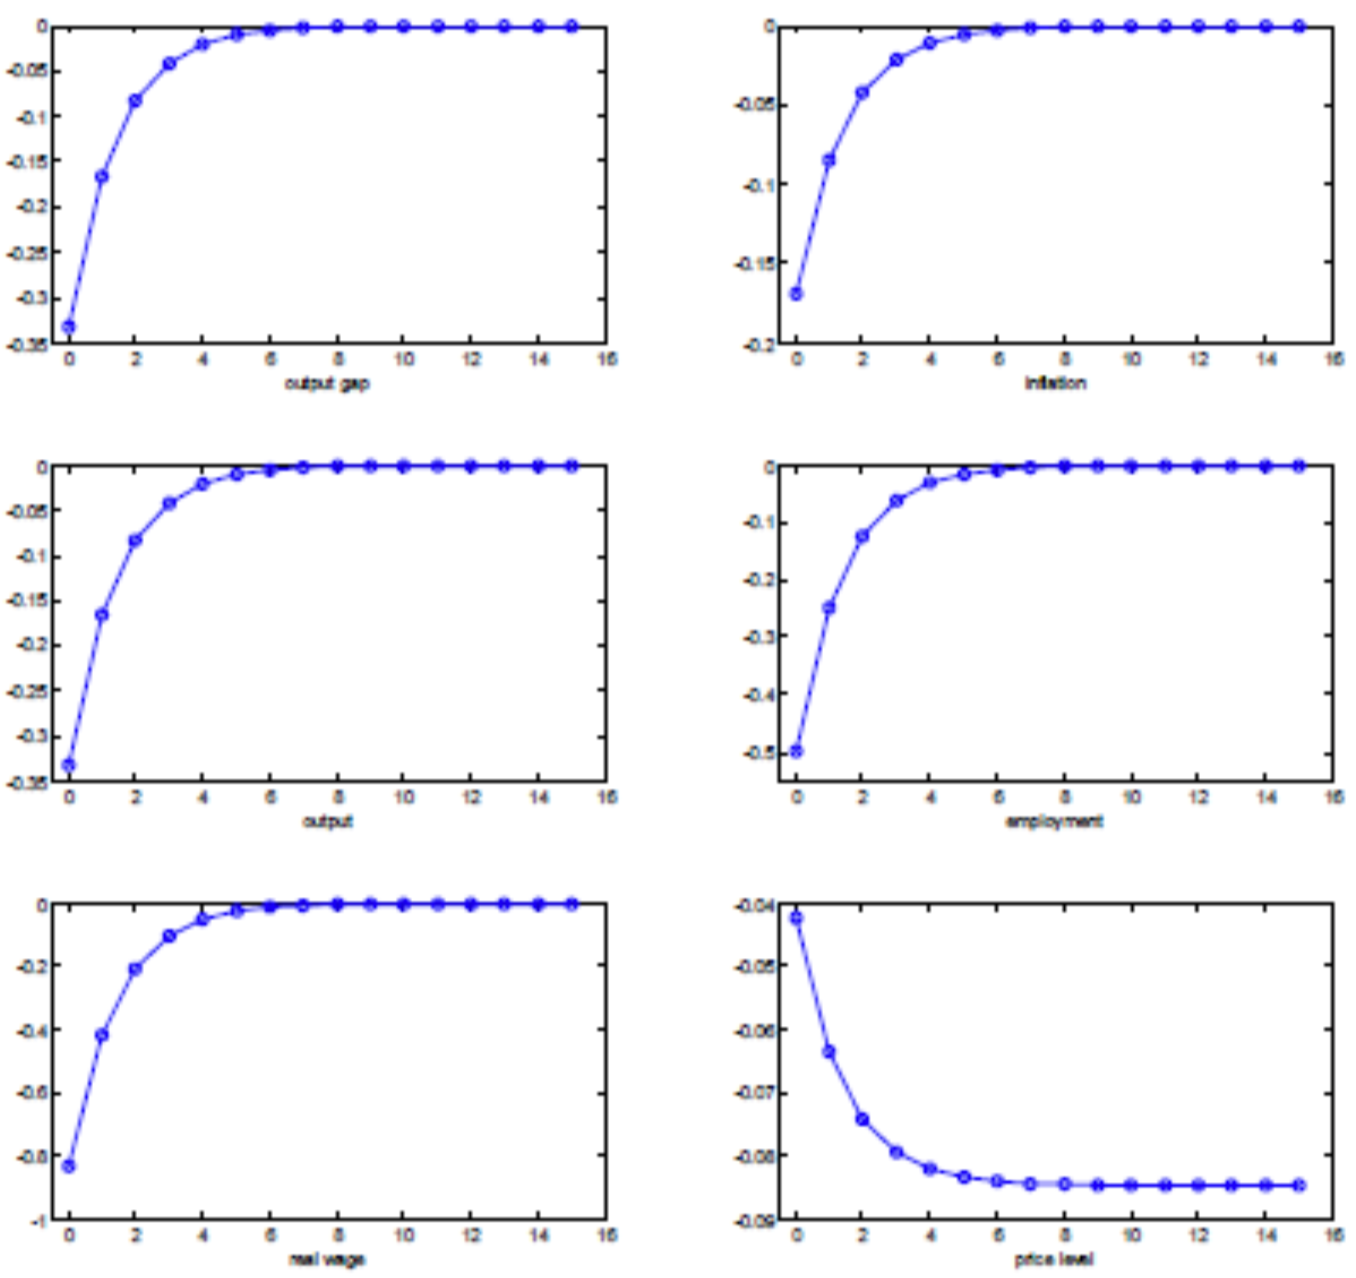
\includegraphics[scale=0.35]{../../Readings/Images/Gali2018irfMP.png}
%\end{frame}
%
%\begin{frame}
%\frametitle{Impulse Response: Discount Rate Shock}
%\centering
%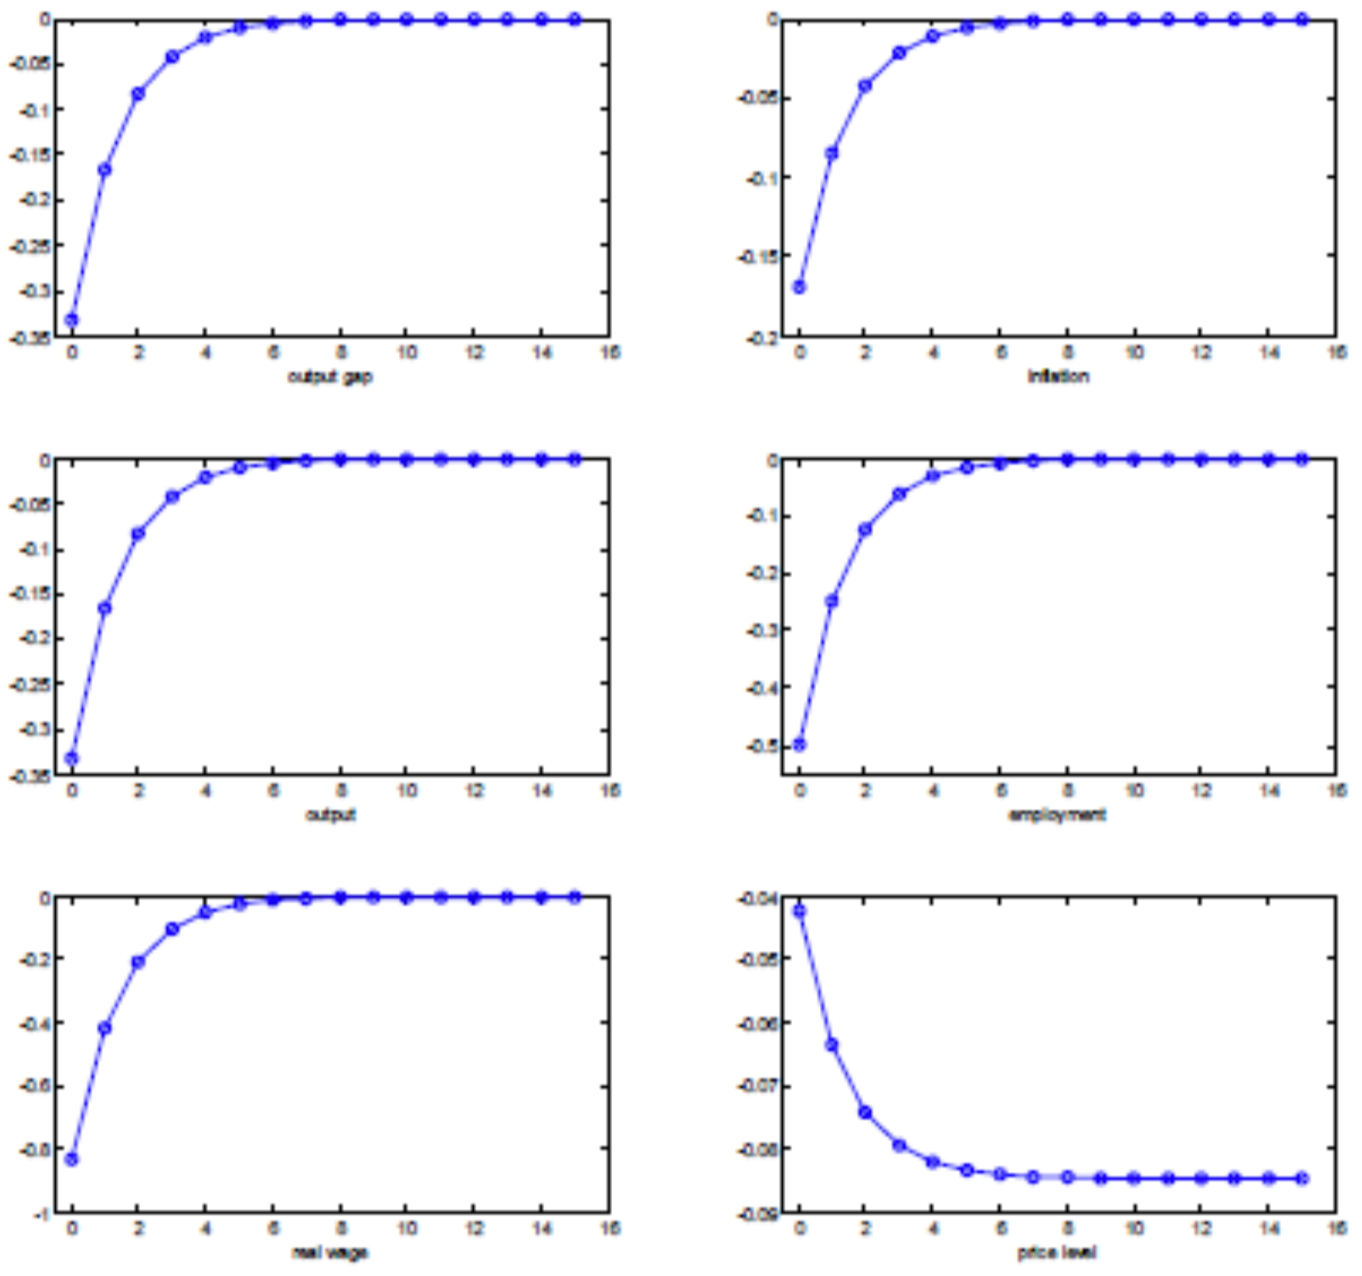
\includegraphics[scale=0.35]{../../Readings/Images/Gali2018irfAD.png}
%\end{frame}
%
%
%\begin{frame}
%\frametitle{Demand Shock vs. Monetary Shock}
%\begin{itemize}
%	\item Demand shocks have an effect on the natural rate of interest, while monetary policy shocks do not.
%	\item Monetary policy shocks lead to changes in the nominal interest rate for a given level of inflation and output, whereas discount factor shocks do not.
%	\item But they go in similar directions.
%	\begin{itemize}
%		\item Monetary policy can fully stabilize \emph{both} output and inflation.
%		\item This turns out to be a special case known as the ``Divine Coincidence.''
%	\end{itemize}
%	\item Note: Impulse responses depend crucially on Central Bank
%response function.
%	\begin{itemize}
%		\item Theme of NK literature.
%		\item Somewhat unsatisfying.
%	\end{itemize}
%\end{itemize}
%\end{frame}
%
%\begin{frame}
%\frametitle{Impulse Response: Tech Shocks}
%\centering
%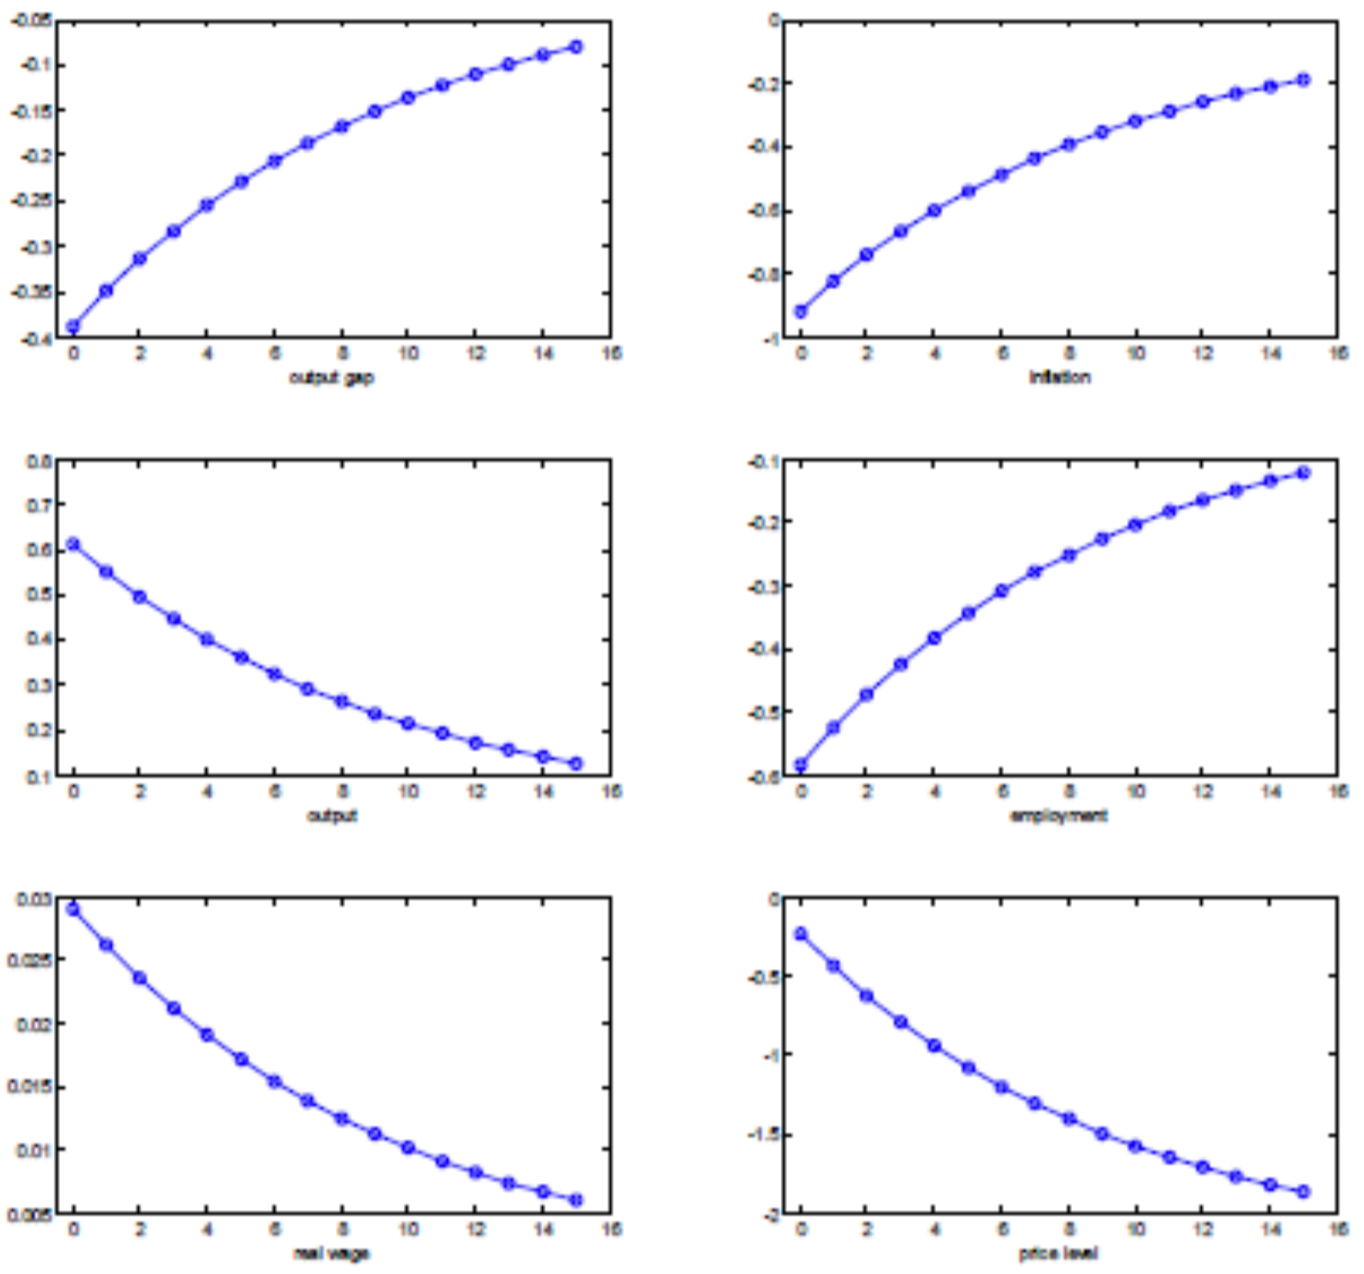
\includegraphics[scale=0.35]{../../Readings/Images/Gali2018irfA.png}
%\end{frame}


\end{document}